\documentclass[a4paper,10pt]{article}
\usepackage[paper=a4paper, hmargin=1.5cm, bottom=1.5cm, top=3.5cm]{geometry}
\usepackage[latin1]{inputenc}
\usepackage[T1]{fontenc}
\usepackage[spanish]{babel}
\usepackage{amssymb}
\usepackage{amsmath}
\usepackage{mathtools}
\usepackage{fancyhdr}
\usepackage{lastpage}
\usepackage{caratula}
\usepackage{verbatim}
\usepackage{xspace}
\usepackage{xargs}
\usepackage{float}
\usepackage{graphicx}
\usepackage{ifthen}
\usepackage[spanish,noline,longend]{algorithm2e}
\usepackage{listings}
\usepackage{braket}
%\usepackage{aed2-tad,aed2-symb,aed2-itef}

\lstset{language=C++, tabsize=4, breaklines=true, breakatwhitespace=true, numbers=left, numbersep=10pt}

\newcommand{\moduloNombre}[1]{\textbf{#1}}

\let\NombreFuncion=\textsc
\let\TipoVariable=\texttt
\let\ModificadorArgumento=\textbf
\newcommand{\res}{$res$\xspace}
\newcommand{\tab}{\hspace*{7mm}}

\newcommandx{\TipoFuncion}[3]{%
  \NombreFuncion{#1}(#2) \ifx#3\empty\else $\to$ \res\,: \TipoVariable{#3}\fi%
}
\newcommandx{\Pre}[1][1=true]{\textbf{Pre} $\equiv$ \{#1\}\\}
\newcommand{\Post}[1]{\textbf{Post} $\equiv$ \{#1\}}
\newcommand{\In}[2]{\ModificadorArgumento{in} \ensuremath{#1}\,: \TipoVariable{#2}\xspace}
\newcommand{\Out}[2]{\ModificadorArgumento{out} \ensuremath{#1}\,: \TipoVariable{#2}\xspace}
\newcommand{\Inout}[2]{\ModificadorArgumento{in/out} \ensuremath{#1}\,: \TipoVariable{#2}\xspace}
\newcommand{\Aplicar}[2]{\NombreFuncion{#1}(#2)}

\newlength{\IntFuncionLengthA}
\newlength{\IntFuncionLengthB}
\newlength{\IntFuncionLengthC}
%InterfazFuncion(nombre, argumentos, valor retorno, precondicion, postcondicion, complejidad, descripcion, aliasing)
\newcommandx{\InterfazFuncion}[9][4=true,6,7,8,9]{%
  \hangindent=\parindent
  \TipoFuncion{#1}{#2}{#3}\\%
%  \textbf{Pre} $\equiv$ \{#4\}\\%
%  \textbf{Post} $\equiv$ \{#5\}%
  \Pre[#4]
  \Post{#5}
  \ifx#6\empty\else\\\textbf{Complejidad:} #6\fi%
  \ifx#7\empty\else\\\textbf{Descripci�n:} #7\fi%
  \ifx#8\empty\else\\\textbf{Aliasing:} #8\fi%
  \ifx#9\empty\else\\\textbf{Requiere:} #9\fi%
}



\newenvironment{Interfaz}{%
  \parskip=2ex%
  \noindent\textbf{\Large Interfaz}%
  \par%
}{}

\newcommand{\Forcond}[2]{
  #1 \textbf{to} #2
}

\newenvironment{Representacion}{%
  \vspace*{2ex}%
  \noindent\textbf{\Large Representaci�n}%
  \vspace*{2ex}%
}{}

\newenvironment{Algoritmos}{%
  \vspace*{2ex}%
  \noindent\textbf{\Large Algoritmos}%
  \vspace*{2ex}%
}{}

%
%\newcommandx{\Signatura}[3][3]{%
%  \NombreFuncion{#1}(#2)
%  \ifx#3\empty\else $\to$ \res\,: \TipoVariable{#3}\fi
%  \\
%}


\newenvironmentx{algoritmo}[6][3,4,5,6]{
  \begin{algorithm}[H]
  \DontPrintSemicolon
  \newcommandx{\Signatura}[3][3]{
    \NombreFuncion{##1}(##2)
    \ifx##3\empty\else $\to$ \res\,: \TipoVariable{##3}\fi
    \\
  }
  \newcommand{\asignar}{$\leftarrow$ }
  \newcommand{\return}{\textbf{return} }
  \newcommand{\Break}{\textbf{break} }
  \Signatura{#1}{#2}[#3]
  \ifx#4\empty\else\Pre[#4]\fi
  \ifx#5\empty\else\Post{#5}\\\fi
  \ifx#6\empty\else\textbf{Complejidad:} #6\\\fi%
}{\end{algorithm} \vspace{0.3cm}}

\newenvironmentx{algoritmosimple}{
  \begin{algorithm}[H]
  \DontPrintSemicolon
  \newcommand{\asignar}{$\leftarrow$ }
  \newcommand{\return}{\textbf{return} }
  \newcommand{\Break}{\textbf{break} }
}{\end{algorithm} \vspace{0.3cm}}


\newcommand{\Titulon}[1]{
  \vspace*{1ex}\par\noindent\textbf{\large #1}\par
}

\newenvironmentx{Estructura}[2][2={estr}]{%
  \par\vspace*{2ex}%
  \TipoVariable{#1} \textbf{se representa con} \TipoVariable{#2}%
  \par\vspace*{1ex}%
}{%
  \par\vspace*{2ex}%
}%

\newboolean{EstructuraHayItems}
\newlength{\lenTupla}
\newenvironmentx{Tupla}[1][1={estr}]{%
    \settowidth{\lenTupla}{\hspace*{3mm}donde \TipoVariable{#1} es \TipoVariable{tupla}$($}%
    \addtolength{\lenTupla}{\parindent}%
    \hspace*{3mm}donde \TipoVariable{#1} es \TipoVariable{tupla}$($%
    \begin{minipage}[t]{\linewidth-\lenTupla}%
    \setboolean{EstructuraHayItems}{false}%
}{%
    $)$%
    \end{minipage}
}

\newcommandx{\tupItem}[3][1={\ }]{%
    %\hspace*{3mm}%
    \ifthenelse{\boolean{EstructuraHayItems}}{%
        ,#1%
    }{}%
    \emph{#2}: \TipoVariable{#3}%
    \setboolean{EstructuraHayItems}{true}%
}

\newcommandx{\RepFc}[3][1={estr},2={e}]{%
  \tadOperacion{Rep}{#1}{boolean}{}%
  \tadAxioma{Rep($#2$)}{#3}%
}%

\newcommandx{\Rep}[3][1={estr},2={e}]{%
  \tadOperacion{Rep}{#1}{boolean}{}%
  \tadAxioma{Rep($#2$)}{true \ssi #3}%
}%

\newcommandx{\Abs}[5][1={estr},3={e}]{%
  \tadOperacion{Abs}{#1/#3}{#2}{Rep($#3$)}%
  \settominwidth{\hangindent}{Abs($#3$) \igobs #4: #2 $\mid$ }%
  \addtolength{\hangindent}{\parindent}%
  Abs($#3$) \igobs #4: #2 $\mid$ #5%
}%

\newcommandx{\AbsFc}[4][1={estr},3={e}]{%
  \tadOperacion{Abs}{#1/#3}{#2}{Rep($#3$)}%
  \tadAxioma{Abs($#3$)}{#4}%
}%

\let\agregar=\argumento

\newcommand{\DRef}{\ensuremath{\rightarrow}}

\pagestyle{fancy}
\thispagestyle{fancy}
\addtolength{\headheight}{1pt}
\lhead{Algoritmos y Estructuras de Datos III}
\rhead{$1^{\mathrm{er}}$ cuatrimestre de 2014}
\cfoot{\thepage /\pageref{LastPage}}
\renewcommand{\footrulewidth}{0.4pt}

%\author{Algoritmos y Estructuras de Datos II, DC, UBA.}
%\date{}
%\title{Tipos abstractos de datos bǭsicos}

\titulo{Trabajo Pr�ctico III - Recuperatorio}
\fecha{ 27 / 6 / 2014}
\materia{Algoritmos y Estructura de Datos III}
\grupo{}
\integrante{Abdala, Leila}{950/12}{abdalaleila@gmail.com}
\integrante{Cingolani, Luis Ignacio}{490/12}{luiscingo@gmail.com}
\integrante{Nale, Sebastian Claudio}{655/11}{sebinale@gmail.com}
\integrante{Straminsky, Axel}{769/11}{axelstraminsky@gmail.com}

\begin{document}

\maketitle
\tableofcontents
\begin{comment}
\newpage
\section{Aclaraciones}
\subsection{Sobre la complejidad }
 En todos los ejercicios trabajamos sobre el Modelo Uniforme. Por lo tanto suponemos en todos los casos que las asignaciones y comparaciones 
 de tipos b�sicos, definici�n de variables, creaci�n de iteradores y operaciones matem�ticas est�ndar tienen una complejidad constante.
 
\subsection{Sobre la implementaci�n }
La carpeta del tp contiene todos los archivos usados en la implementaci�n del problema, tambi�n contiene una subcarpeta llamada Tests, que contiene todo lo relativo al testeo del ejercicio. La carpeta de Tests contiene los generadores de instancias aleatorias, la experimentaci�n, y las comparaciones entre heur�sticas, que fueron usadas para crear los gr�ficos.
 
Tambi�n se adjuntan Makefile's para asegurar que el proceso de compilaci�n sea el mismo. 
 
 \subsection{Sobre la ejecuci�n }
 Para la ejecuci�n de los ejecutables, debe pasarse como par�metro un 1 o un 0 que indica si debe 
 tomar mediciones o no. 1 significa que si, 0 que no debe hacerlo, adem�s deben pasarse par�metros adicionales indicando que heuristica se desea aplicar(exacto, goloso, local y grasp). Finalmente, se debe usar el operador de redirecci�n <, seguido del nombre del archivo que contiene las instancias de test.
 La ejecuci�n de los generadores de instancias es directa, luego se pide ingresar los par�metros por consola, durante la ejecuci�n.  
 
  
 \subsection{Sobre la experimentaci�n }
A fin de reducir el $ruido$, ejecutamos 20 veces la resoluci�n de la misma instancia, y tomamos el tiempo final como
el promedio de los tiempos sumados.
\subsubsection{Medici�n de Tiempos}
Para realizar la medici�n de tiempos, utilizamos el tipo timespec.



\newpage
\section{Descripci�n de situaciones reales}
\subsection{Ejemplo 1: Viaje en auto} Queremos minimizar la distancia recorrida sin quedarte sin nafta, 
teniendo un tanque con k cantidad de nafta que no puede ser recargado (por falta de presupuesto).
\paragraph{Modelado en un grafo} Los nodos son las ciudades (pueblos, estaciones, lugares tur�sticos o cualquier cruce de caminos).
Las aristas son las rutas que unen ciudades. El peso $w_1$ es la cantidad de nafta necesaria para 
recorrer ese tramo, y $w_2$ la distancia entre las ciudades. N�tese que no son dependientes $w_1$ y $w_2$ entre si; podemos necesitar mas
nafta para una distancia mas corta si, 
por ejemplo, tenemos que subir una cuesta o ir a una velocidad m�xima determinada.

\subsection{Ejemplo 2: S�per Minis-Vacaciones} Fuckensio lleva toda su vida ahorrando para irse de vacaciones a $Wolololandia$ y junto $K$ 
cantidad de dinero, del que destino $K'$ para el viaje de ida.
Como a Fuckensio le pagan por hora de trabajo independientemente del horario en que la realice, decidi� tomarse solo unos d�as de vacaciones, 
teniendo en cuenta hasta la ultima hora del 
viaje, por lo que necesita llegar
a la $Wolololandia$ lo mas r�pido posible, porque Fuckensio es pobre. Luego, usaremos este algoritmo para ayudarle a elegir el viaje �ptimo.
\paragraph{Modelado en un grafo} Los nodos son las ciudades donde empiezan y terminan los vuelos de la aerol�nea, que son representados por 
las aristas. El peso $w_1$ representa 
el costo del viaje y el peso $w_2$ representa el tiempo que dura el vuelo. Para simplificar el problema, asumimos que Fuckensio es una 
persona muy $Snob$ y como no quiere compartir 
el avi�n con nadie,alquilo un avi�n y pilotos privados por viaje.
Es decir, que puede partir inmediatamente luego de llegar al aeropuerto.

\subsection{Ejemplo 3: Pokemoon recargado.} Nuestra historia comienza en un momento critico del siglo 21. Un grupo anarquista llamado 
``Los Frikis Originales'', descontentos con 
la facilidad de los juegos actuales, realizo una protesta sobre los mismos. Dicho grupo determino que el mejor juego de la historia 
era el Pokemoon, por lo que 
comenz� a enviar cartas (y mails, y bombas) a las instalaciones de la compa��a GameBoi exigiendo nuevas versiones del juego Pokemoon
- Hoja Verde. Este desmadre de ``frikismo''
llego a tal nivel que los llamados ``Frikis Originales'' rastrearon a cada uno de los programadores del juego original y enviaron sus
reclamos a las casas de los mismos. 

Esto molesto a los programadores. Por lo tanto, anunciaron que crear�an un reto final, s�per dif�cil, que solo los jugadores veteranos
podr�an superar. Ahora bien, dichos programadores no
ten�an ganas de hacer 
un nuevo juego, por lo que se limitaron a aumentar la dificultad del original. Lograron esto, mediante el borrado de pedazos el c�digo.
Es decir, le sacaron jugabilidad al juego.

Ahora el nuevo reto consiste, obviamente, en ganar la Liga Pokemoon. Sin embargo, las reglas han cambiado. Ahora no existen los hospitales
Pokemoon, ni hay posibilidad de capturar o hacer evolucionar a 
los pokemoon, dado que ya no hay pokemoon salvajes (porque fueron todos capturaron por los frikis originales en la primera versi�n
del juego). Tampoco hay misiones extras. 
Lo que esto significa, es que debes
pasar por los gimnasios, uno tras otro, y llegar a la final, sin poder curar nunca a tus pokemoon. Y como que los programadores estaban 
realmente enfadados, decidieron aumentar la dificultad de la final, 
para que todos los jugadores llegaran con relativa facilidad hasta ella, pero ninguno pudiera pasarla.

Cuando el nuevo juego salio a la venta, nuestro protagonista Bill, un miembro de los ``Frikis Originales'', muy ilusionado descargo 
(ilegalmente) e instalo dicho juego a primera hora de su
ma�ana. Cuando se dispon�a a jugar, luego de finalizada la instalaci�n una hora mas tarde, apareci� su madre record�ndole que deb�a 
trabajar para independizarse, a sus 
cuarenta a�os, y que a las 17:00 hs pm tenia que presentarse en el McKonalls de junto para 
cumplir su horario laboral. Dado esto, a Bill le restaban 3 horas para terminar su juego, si quer�a llegar a tiempo.

Es por esto que Bill se encontraba en un dilema, pues quer�a terminar el juego y estimaba que la final pod�a costarle media hora de 
juego. Siendo tan friki como es, Bill puede estimar cuanto
tiempo le va a costar y llegar y
vencer en cada gimnasio con los pokemoon de que dispone, y cuan heridos van a terminar los mismos despu�s de cada combate. Como no sabe 
nada sobre la final, lo que Bill quiere lograr es minimizar el da�o total sufrido por el conjunto de sus pokemoon. 

Ahora bien, como Bill es un gran amigo nuestro, pues ha cuidado de nuestros pokemoon en su computadora durante mucho tiempo, 
decidimos ayudarlo modelando su problema con CACM. 

\paragraph{Modelado en un grafo} Los nodos son los gimnasios y las aristas representan los caminos entre ellos, si es posible llegar 
de uno a otro. El peso $w_1$ representa 
el tiempo que le lleva, al personaje de Bill, ir de un gimnasio a otro y vencer en dicho gimnasio. El peso $w_2$ representa el da�o 
que reciben los pokemoon en conjunto al finalizar cada combate.
La cota son las dos horas que le restan, pues hemos gastado media en escribir el grafo asociado al problema.

\paragraph{Problema adicional:} �A que hora comienza la ma�ana de Bill?



\newpage
\section{Algoritmo exacto}
\subsection{Descripci�n del algoritmo}
Este algoritmo parte de un camino inicial $C$ vac�o. 
Luego, toma el nodo inicial $v$, recorre las aristas adyacentes cuyos nodos incidentes no est�n 
marcados como visitados. Para cada arista, chequea que al agregarla siga teniendo una soluci�n factible. Si es as�, y el otro extremo 
$w$ de la arista no est� marcado como visitado, 
agrega la arista, se para en ese nodo, y chequea si es igual al nodo final. Si lo es, compara el camino obtenido con $C$,
y almacena
en $C$ el de menor peso respecto a W2. Luego marca como nodo inicial a $w$, marca como visitado a $v$ y repite recursivamente
el proceso. Esto es b�sicamente una resoluci�n con backtracking. 


\subsection{Complejidad}

\begin{algoritmo}{HallarCaminoMinimoAcotadoPorK}{grafo, verticeActual, verticeDestino, K, camino, caminoMinimo}
\;
  Visitar(verticeActual, grafo)	\tcc*{$O$(1)}\;
  
  \For(\tcc*[f]{$O$(|AristasIncidentesA(verticeActual, grafo)| * )}){\Forcond{e \asignar AristasIncidentesA(verticeActual, grafo)}}{
  
    vecino $\leftarrow$ ObtenerVerticeVecinoA(verticeActual, e) \tcc*{$O$(1)}\;
  
    \If(\tcc*[f]{$O$(1)}){PesoTotalEnW1(camino) + PesoW1(e) < K $\wedge$ $\neg$FueVisitado(vecino)}{
    
      \uIf(\tcc*[f]{$O$(1)}){vecino $\not=$ verticeDestino}{ \tcc*{$O$(1)}
	
	AgregarArista(e, camino)	\tcc*{$O$(1)}\; 
	HallarCaminoMinimoAcotadoPorK(grafo, vecino, verticeDestino, K, camino, caminoMinimo)	\;
	RemoverArista(e, camino)	\tcc*{$O$(1)}\;
             
      }\Else{
      
	AgregarArista(e, camino)	\tcc*{$O$(1)}\;
	caminoMinimo \asignar ObtenerElCaminoMinimoEntre(camino, caminoMinimo)	\tcc*{$O$(|camino|)}\;
	RemoverArista(e, camino)	\tcc*{$O$(1)}\;
      
      }
      
    }
    
  }
  
  Desvisitar(verticeActual, grafo)	\tcc*{$O$(1)}\;
\end{algoritmo}

Complejidad Total: Este algoritmo es recursivo. Para cada nodo recorre a lo sumo todas las aristas, pero podemos acotar esto sabiendo 
que si visitamos un nodo en la K-esima llamada, ya habremos 
marcado como visitados a k nodos antes, por lo que solo recorrer�a en el peor caso $n-k$ aristas, porque solo puede tener $n-1$ aristas
incidentes, y as� recursivamente, 
donde $n$ es la cantidad inicial de nodos. Luego la complejidad de este algoritmo es
$\Pi_{k=1}^{n} n-k $. Por lo tanto, la complejidad en el peor caso de este algoritmo es $(n-1)!$.

\subsection{Experimentaci�n}

Para la medici�n de tiempo de este algoritmo, creamos un generados de grafos aleatorio. El gr�fico 
que presentemos esta contantizado, es decir,
las mediciones fueron divididas por la complejidad que calculamos en el punto anterior. Ac� esperar�amos observar 
una constante pero 
dado que la complejidad de este algoritmo es factorial, las muestras que podemos son muy peque�as, por lo que el 
gr�fico no puede presentar las 
suficientes muestras para que la curvatura de la funci�n tienda a algo. Sin embargo, podemos ver que el gr�fico se 
mantiene cerca del eje x, lo que 
nos indica que claramente la complejidad esta acotada por la calculada.

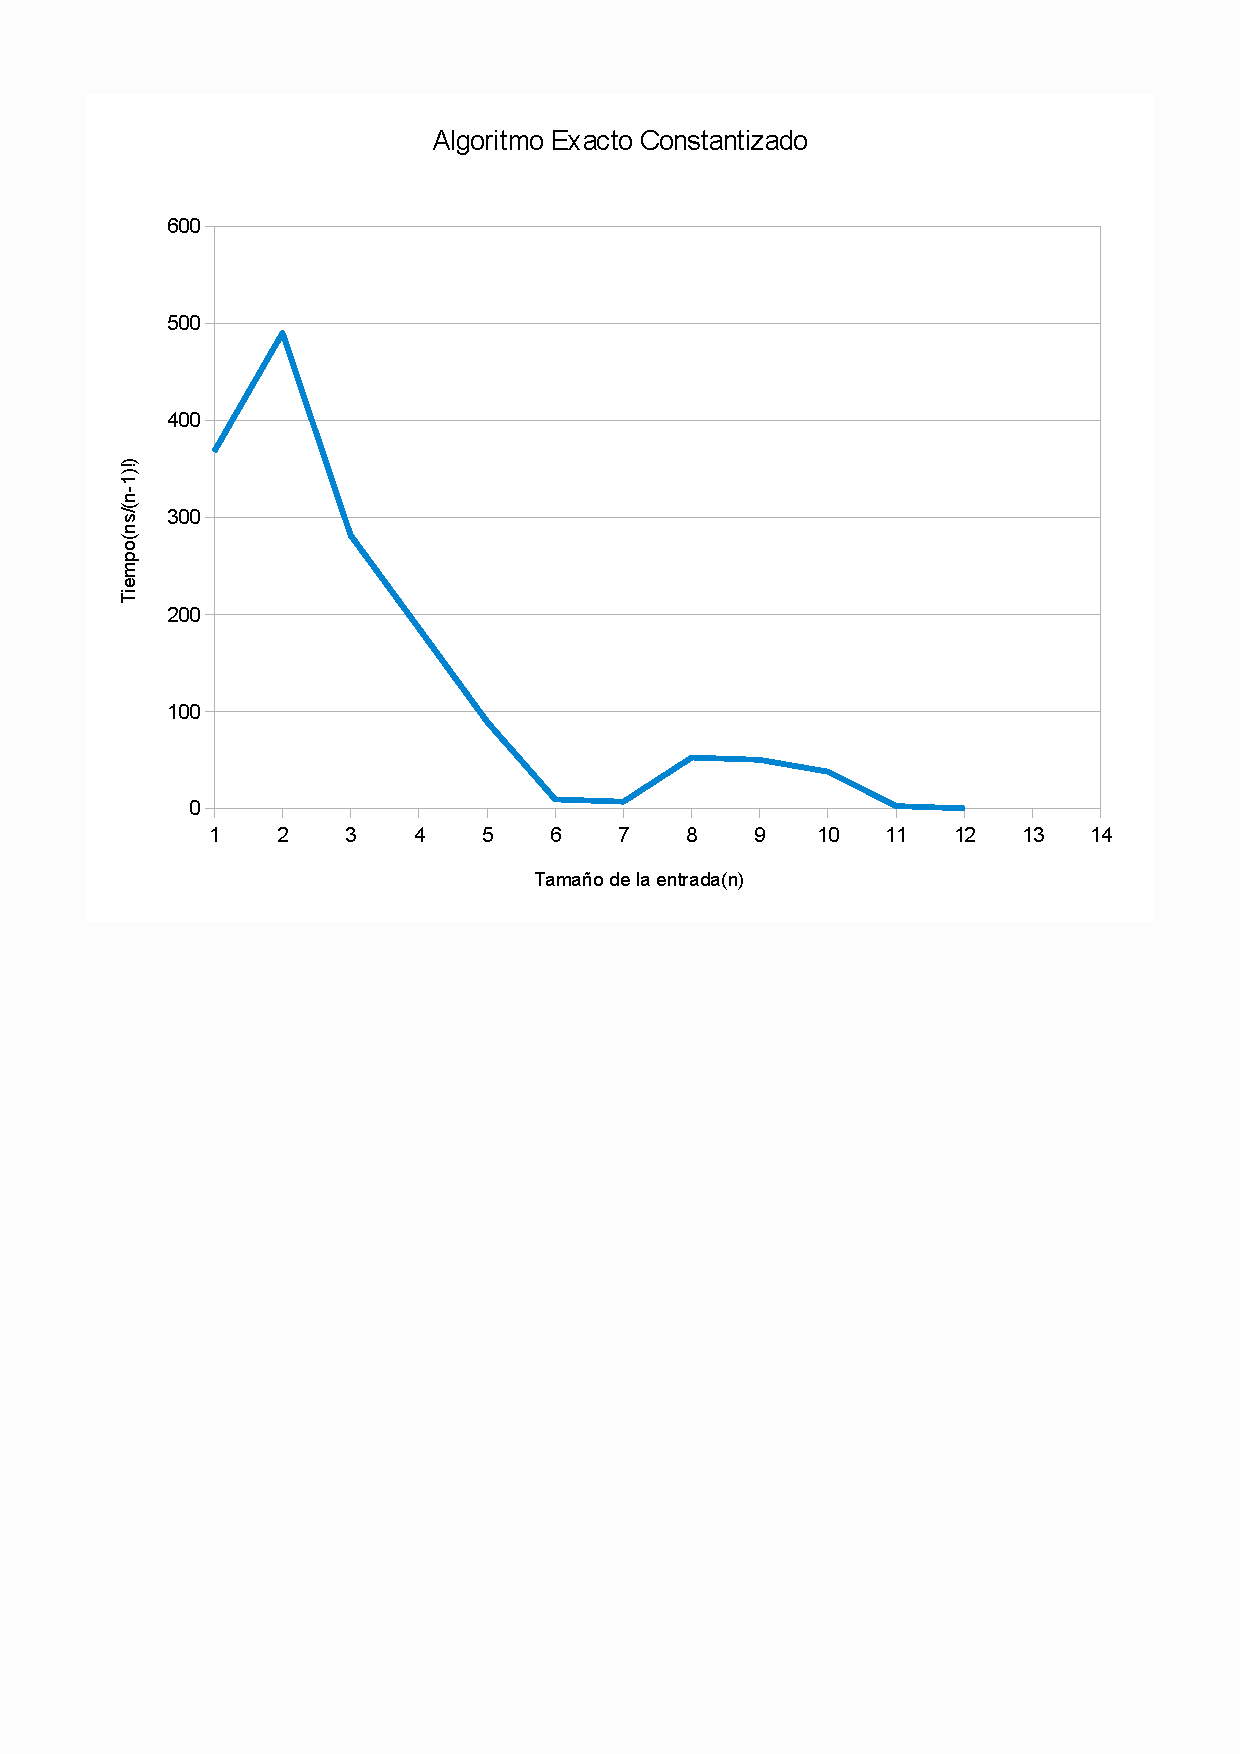
\includegraphics[width=1\textwidth]{exacto_grafico.pdf}[!]


\newpage
\section{Heur�stica Constructiva Golosa}
\subsection{Descripci�n del algoritmo}
El algoritmo consiste en, dado un grafo $G$, las funciones de peso de aristas W1 y W2, un v�rtice de inicio $u \in G$, un
v�rtice de destino $v \in G$, y un entero que representa la cota de el peso W1, $K$.
Generamos dos caminos, MinW1 y MinW2, que minimizan los pesos W1 y W2 entre $u$ y $v$. Utilizo Dijkstra para generar estos 
dos caminos, y como Dijkstra que representa la parte golosa de esta heur�stica.
Luego para el camino MinW2 veo su peso en funci�n de W1, si su peso es menor que $K$ entonces esta es la soluci�n �ptima, 
pues no existe un camino mas chico en funci�n de W2 que cumpla que su peso en funci�n de W1 sea menor que $K$.
Si esto no sucede entonces tomo el camino MinW1 y veo su peso en funci�n de W1, si su peso es mayor o igual que $K$ entonces
no existe soluci�n, pues todos los caminos son mayores que $K$. En caso contrario devuelvo este camino, ya que es un camino 
valido ente $u$ y $v$ que no supera la cota.
Este algoritmo me asegura que si existen caminos que cumplen que su peso W1 < K entonces va a devolver un camino valido.


\subsection{Pseudoc�digo y Complejidad}
\begin{algoritmo}{HallarCaminoGoloso}{grafo, verticeInicio, verticeDestino, K, camino} [][][][$O$(mlog(n))]
\;
  Camino res = MinimoAbsolutoSegunPeso(grafo, inicio, destino, K, funcionPesoW2) \tcc*{$O$(mlog(n))}
  \If (\tcc*[f]{$O$(1)}) {res.Longitud() > 0}{
   return res \tcc*{$O$(n)}
  }
  res = MinimoAbsolutoSegunPeso(grafo, inicio, destino, K, funcionPesoW1) \tcc*{$O$(mlog(n))}
  return res \tcc*{$O$(n)}
\end{algoritmo}

\begin{algoritmo}{MinimoAbsolutoSegunPeso}{grafo, inicio, destino, K, funcionPeso}[][][][$O$(mlog(n))]
	Camino res = grafo.DijkstraEntre(inicio, destino, funcionPeso) \tcc*{$O$(mlog(n))}
	\If (\tcc*[f]{$O$(1)}) {res.PesoTotalEnW1() < K}{
		return res \tcc*{$O$(n)} 
	}
	\Else{
		return CaminoVacio \tcc*{$O$(n)}
	}
\end{algoritmo}

\paragraph{Aclaraciones:} 
Dado un grafo G, n es la cantidad de vertices y m es la cantidad de aristas del grafo.

Retornar un camino se hace por copia, por lo que la complejidad al devolverlo es el tama�o del camino, como Dijktra
devuelve caminos simples la cantidad de elementos del camino sera a lo sumo n-1, asi que la complejidad es $O$(n).

Dijkstra esta implementado sobre heap, sin ninguna modificaci�n que pudiera cambiar su complejidad temporal, por lo que
DijkstraEntre, que toma una funci�n de peso, dos puntos de un grafo y encuentra el camino minimo segun la funcion, utilizando
Dijkstra, sera $O$(mlog(n)

\subsection{Casos Patol�gicos}
Cualquier grafo en el que, para el camino creado usando la funci�n de peso W2, su peso en W1 
sea mayor que K, y que exista un camino que minimiza W2 
que es menor que el camino creado usando la funci�n de peso W1.

\subsection{Experimentaci�n}

\subsubsection{General}
Para la experimentaci�n general usamos el mismo generador aleatorio que el caso exacto, medimos los tiempos de ejecuci�n y los dividimos por la
complejidad calculada en el punto anterior en funci�n del tama�o de la entrada, antes de gr�ficar. Lo que observamos en el gr�fico es que la 
curva oscila entre un intervalo acotado. Podemos deducir entonces que el la complejidad es acertada, pues podemos acotarlo por una constante 
mayor
a nuestro intervalo.

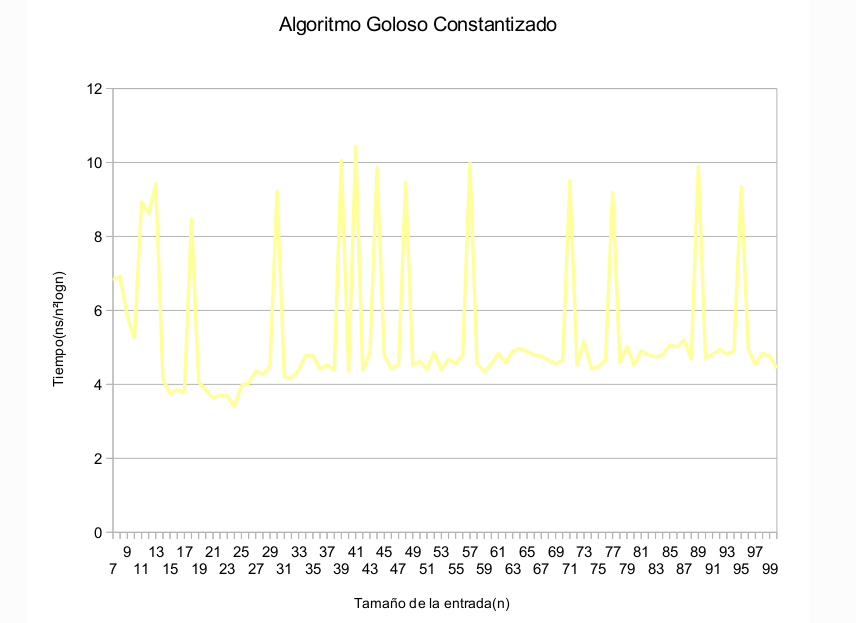
\includegraphics[width=1\textwidth]{goloso_grafico.png}

\subsubsection{Casos Patol�gicos}
Para la experimentacion de los casos patologicos, generamos un test que nos da grafos completos a los que a�adimos dos caminos, uno que 
miniza el peso $w_1$ 
y maximiza el peso $W_2$, y al revez para el otro. El hecho de que sean completos es por simplicidad en la implementacion. 
En el grafico presentamos la 
comparacion de los resultados contra el algoritmo exacto.

Podemos observar que los caminos difieren en la mayoria de los casos, y en los casos que no, se debe a que hay un camino dentro del subgrafo completo
de peso equivalente al optimo que agregamos.

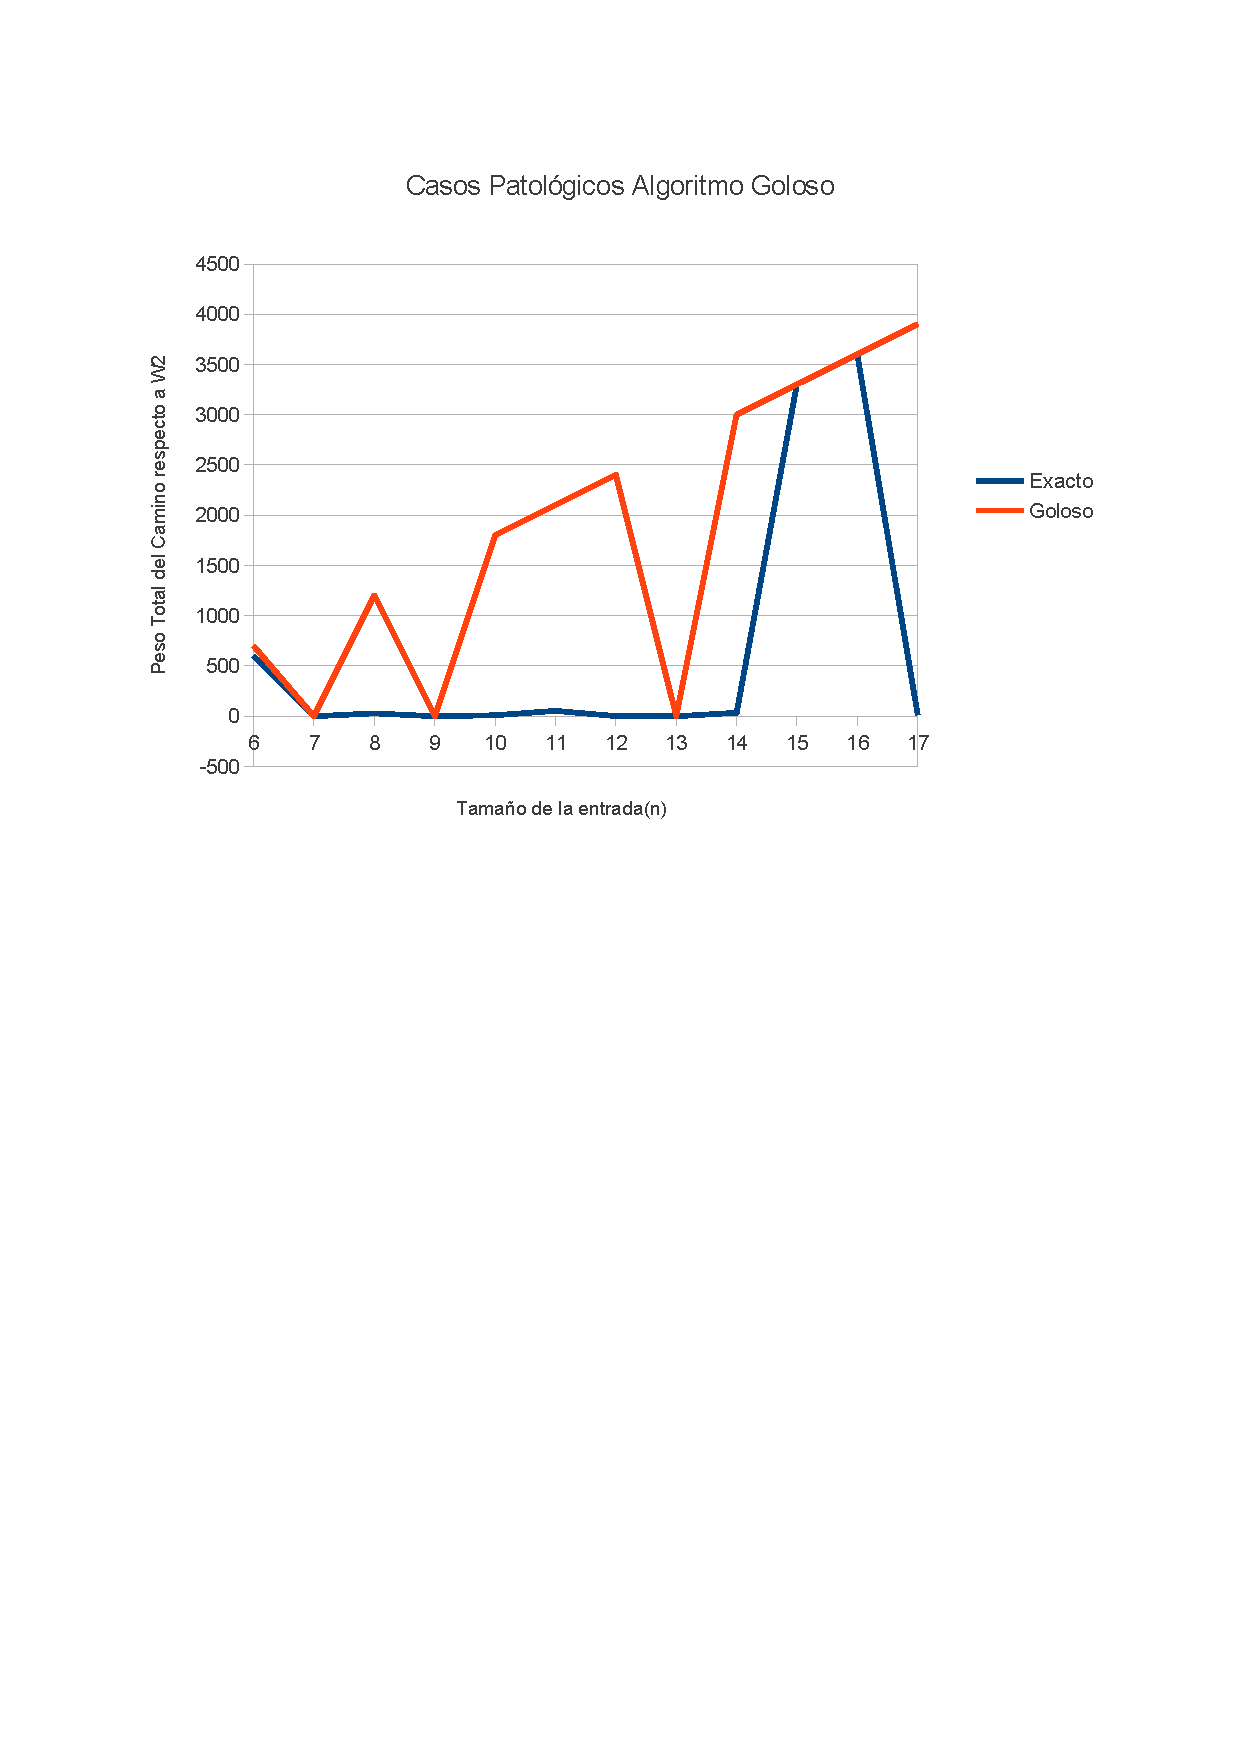
\includegraphics[width=1\textwidth]{casos_patologicos_goloso.pdf}


\newpage
\section{Heur�stica de B�squeda Local}
%busqueda local
\subsection{Descripci�n del algoritmo}

\subsubsection{Soluci�n inicial}

La soluci�n inicial, en este caso, se toma como el camino m�nimo, para $w_2$, entre los dos nodos. Sabemos que si el peso del camino, 
para $w_1$, es menor a la cota, entonces la soluci�n inicial es tambi�n la �ptima, por lo que podemos devolverla y finalizar el algoritmo sin 
necesidad de recorrer la vecindad. En caso contrario, tomamos el camino m�nimo para $w_1$ y, si el peso de este es menor que la cota K, 
utilizamos
este camino como soluci�n inicial. Si no cumple con la cota, al ser el m�nimo camino respecto a $w_1$, entonces ninguno la cumple, y por lo tanto la 
instancia del problema no tiene soluci�n, por lo que devolvemos el camino vac�o.

\subsubsection{Vecindad}
Definimos como vecinos de una soluci�n, cuyo camino llamamos $C$, aquellas soluciones que difieren en a lo sumo un camino m�nimo para $w_2$,
siempre y cuando, estas ``soluciones'' est�n acotadas correctamente para $w_1$.
Es decir, para todo par de nodos, $C_i$ y $C_j$, consideramos como  ``vecino'' de $C$ al camino $C'$ = $C_1$ .. $C_i$ $C_{min}$ $C_j$ .. $C_k$, 
donde k es la longitud de $C$, $C_n$ el n-esimo nodo de $C$, y $C_{min}$ el camino �ptimo entre $C_i$ y $ C_j$. Luego, entre estos ``vecinos'', 
tomamos como verdaderos vecinos a aquellos ``vecinos'' que cumplan la cota para $w_1$.


Para simplificar el proceso, recorreremos la vecindad en orden. Vamos a considerar los caminos �ptimos entre un nodo $v$ y todos los dem�s, 
donde $C_k$ es el primer nodo que nos genera una mejora mediante este proceso. 
Es decir, tomamos el nodo $C_k$, calculamos el camino m�nimo para $w_2$ para todos los nodos del camino, si genera una mejora, actualizamos 
el camino eligiendo el vecino �ptimo, sino, repetimos el proceso con el nodo $C_{k+1}$ hasta llegar al final.


\subsubsection{Estructura de la implementaci�n}
El algoritmo consiste en, dada una soluci�n inicial, recorrer la vecindad de la misma y tomar la mejor soluci�n. Sin embargo, en cada iteraci�n
nos ``olvidamos'' del pedazo de camino que ya modificamos, es decir, si en un paso de la iteraci�n optimizamos el camino hasta el nodo $C_i$, 
en el siguiente paso de la iteraci�n vamos a correr el algoritmo para el camino formado por $C_{[i..k]}$, donde k es la longitud de $C_K$.

Esto es v�lido, pues no puede ser que yo consiga un mejor camino considerando cada nodo del camino $C_{cambiado}$=$C_1$..$C_i$. Esto se debe a 
que para cada nodo $v$ del 
camino, tomo el camino m�nimo entre $C_1$ y $v$, luego, si existiese un camino $C'$ entre $w \neq C_1$ y $v$, con $w \in C_{cambiado}$, que
mejorara mi soluci�n
 $C$ original m�s que $C_{cambiado}.. C_{[i..k]}$, podr�a construir un camino $C''$ entre $C_1$ y $v$, yendo de a trav�s de $C_{cambiado}$ a 
 $w$, y luego de manera �ptima a $v$.
 Luego, tendr�a que haber hallado el camino $C''$ para llegar a $v$ o uno mejor (pues 
 chequeo para cada nodo el �ptimo), y por lo tanto, deber�a haber sido comparado dentro de la vecindad. Luego, como $C''$ mejora m�s la soluci�n,
 $C''$ deber�a haber sido el camino elegido para optimizar. Los cual es absurdo,
 porque partimos del hecho de que $C_{cambiado}$ me daba la mejor soluci�n para los caminos iniciados en $C_1$. 

Las iteraciones contin�an hasta que se terminen los nodos del camino. Luego devolvemos el camino reconstruido. 


\subsection{Pseudoc�digo y Complejidad}

%%                INDENTAR ESTA MIERDA

\begin{algoritmo}{Busqueda Local}{grafo, verticeActual, verticeDestino, K}

caminoInicial \asignar GenerarSolucionInicial(grafo, u, v, K) \tcc*{$O$($n$)}
 
\If(\tcc*[f]{$O$($1$)}){Longitud(caminoInicial) == 0}{
   return camino vacio
}

iter \asignar IteradorDeAristasAlInicioDe(caminoInicial)  \tcc*{$O$($n$)}
 
 \While(\tcc*[f]{$O$($n� + nmlogn$)}) {iter no llego al final} {
    
    x \asignar ObtenerVerticeIzquierdo(AristaActual(iter)) \tcc*{$O$($1$)}
    mejorCaminoMinimoEnVecindad \asignar HallarMejorCaminoEnVecindadDeX(grafo, caminoInicial, x, iter, K) \tcc*{$O$($n� + mlogn$)}
    
    \uIf(\tcc*[f]{$O$($1$)}){Longitud(mejorCaminoMinimoEnVecindad) != 0}{
      MejorarCaminoInicial(caminoInicial, mejorCaminoMinimoEnVecindad, iter, x)  \tcc*{$O$($n$)}
      }\Else{
      Avanzar(iter)	\tcc*{$O$($1$)}
      }
 }

 return caminoInicial
\end{algoritmo}

Complejidad Total: $O$($n� + nmlogn$)

~\\
\newline
\begin{algoritmo}{HallarMejorCaminoEnVecindadDeX}{grafo, caminoInicial, x, iter, K}

 mejorCaminoMinimoEnVecindad \asignar Vacio()	\tcc*{$O$($1$)}
 iter2 \asignar iter	\tcc*{$O$($1$)}
 arbolDeDistancias \asignar Dijkstra(grafo, x, PesoW2)  \tcc*{$O$($mlogn$)}\;
 
  \While(\tcc*[f]{$O$($n�$)}) {iter2 no llego al final} {
    y \asignar ObtenerVerticeDerecho(AristaActual(iter2))	\tcc*{$O$($1$)}
    caminoMinimoEntreXeY \asignar ArmarCaminoEntre(x, y, arbolDeDistancias, grafo)	\tcc*{$O$($n$)}
    pesoW1DeLasAristasEntreXeY \asignar ObtenerPesoDeLasAristasEntre(x, y, PesoW1, caminoInicial) \tcc*{$O$($1$)}
    pesoW2DeLasAristasEntreXeY \asignar ObtenerPesoDeLasAristasEntre(x, y, PesoW2, caminoInicial) \tcc*{$O$($1$)}\;
    \If(\tcc*[f]{$O$($1$)}){PesoTotalEnW1(caminoInicial) + PesoTotalEnW1(caminoMinimoEntreXeY) - pesoW1DeLasAristasEntreXeY < K \; $\wedge$ PesoTotalEnW2(caminoMinimoEntreXeY) < pesoW2DeLasAristasEntreXeY}{
       
       ObtenerCaminoMinimoEntre(caminoMinimoEntreXeY, mejorCaminoMinimoEnVecindad) \tcc*{$O$($n$)}

    }
    
  }
 
\end{algoritmo}

Complejidad Total: $O$($n� + mlogn$)

~\\
\newline
\begin{algoritmo}{MejorarCaminoInicial}{caminoInicial, mejorCaminoMinimoEnVecindad, iter, x}

 iterFinalCaminoMinimo \asignar CrearIteradorAlFinal(mejorCaminoMinimoEnVecindad) \tcc*{$O$($1$)}
 finalCaminoMinimo \asignar ObtenerVerticeDerecho(AristaActual(iterFinalCaminoMinimo)) \tcc*{$O$($1$)}
 AvanzarHasta(finalCaminoMinimo, iter) \tcc*{$O$($n$)}
 EliminarAristasEntre(x, finalCaminoMinimo, caminoInicial) \tcc*{$O$($n$)}
 UnirCon(mejorCaminoMinimoEnVecindad, caminoInicial) \tcc*{$O$($n$)}
 
\end{algoritmo}

Complejidad Total: $O$($n$)


~\\
\newline



\subsection{Casos Patol�gicos}

En aquellos grafos donde exista un camino $C_{max(w_1), min(w_2)}$ y un $C_{min(w_1+1), min(w_2+1)}$ aislado, es decir, que no comparta 
vertices con cualquier otro caminos entre los nodos inicial y final, con 
$k$ la cota para $w_1$, $max(w_1)>k$ y $min(w_1+1)\leq k$ y empiece el algoritmo con un $C_{inicial} \neq C_{min(w_1+1), min(w_2+1)}$ 
entonces esta heur�stica no tiene forma de hallar este camino �ptimo $C_{min(w_1+1), min(w_2+1)}$, 
que podr�a o no ser el �nico, dependiendo si hay mas de una soluci�n �ptima. 

Esto se debe a que cuando busque los caminos m�nimos, para $w_2$, entre todo par de nodos del camino inicial, no encontrara a 
$C_{min(w_1+1), min(w_2+1)}$ pues no es el m�nimo, sin embargo, si es el m�nimo que cumple las condiciones.

Esto puede generalizarse para cualquier grafo que tenga un camino $C$ soluci�n �ptima que sea de peso mayor para $w_2$ 
a todos los caminos m�nimo para $w_2$ que no cumplan la cota, y de peso menor para todos los dem�s que si, y sin embargo no tenga nodos 
en com�n con el camino inicial.  


\subsection{Experimentaci�n}

\subsubsection{General}
Para la experimentaci�n general usamos el mismo generador aleatorio que el caso exacto, medimos los tiempos de ejecuci�n y los dividimos por la
complejidad calculada en el punto anterior en funci�n del tama�o de la entrada, antes de gr�ficar. Lo que observamos en el gr�fico es que la 
curva tiende a cada vez mas a cero. Esto nos muestra, emp�ricamente, que la complejidad es, en el caso promedio, menor que la esperada, lo que 
implica que solo en el peor caso se alcanza realmente la cota.

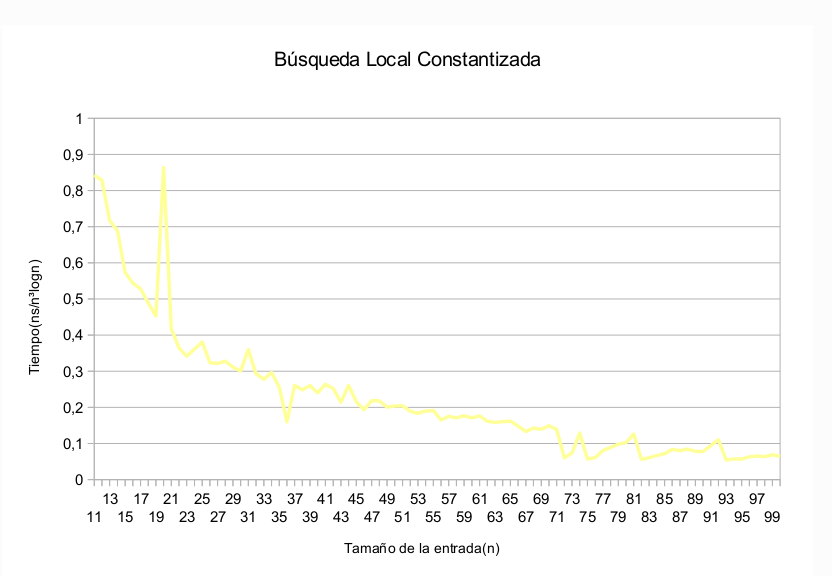
\includegraphics[width=1\textwidth]{busqueda_local_grafico.png}

\subsubsection{Casos Patol�gicos}
Para la experimentacion de los casos patologicos, generamos un test que nos da grafos completos a los que a�adimos los camino que describimos en 
an la subseccion 5.3. El hecho de que sean completos es por simplicidad en la implementacion. En el grafico presentamos la 
comparacion de los resultados contra el algoritmo exacto.

Podemos observar que los caminos difieren en la mayoria de los casos, y en los casos que no, se debe a que hay un camino dentro del subgrafo completo
de peso equivalente al optimo que agregamos.

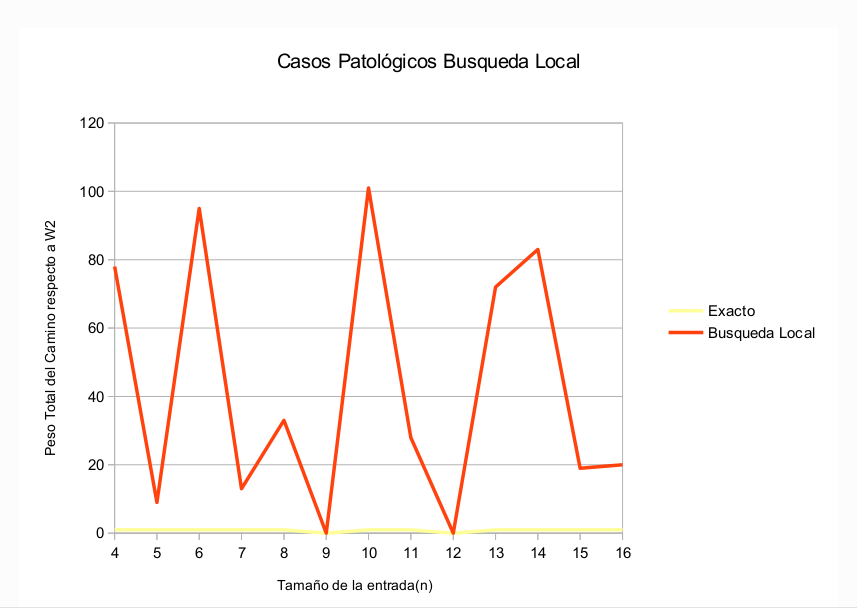
\includegraphics[width=1\textwidth]{casos_patologicos_BL.png}



\newpage
\end{comment}

\section{Informe de modificaciones}
Solo se modifico el item 5.

\section{Heur�stica GRASP}
\subsection{Descripci�n del algoritmo}
El algoritmo corre Dijkstra entre $d$ y todos los dem�s nodos para ambos pesos por separado, obteniendo as� el peso de cada camino m�nimo. 
Estos pesos m�nimos se guardan en dos tablas de distancias $tDW1$ y $tDW2$.

Luego de hacer esto generamos un camino aleatorio como base para poder utilizar la b�squeda local sobre �l, esto se logra de la siguiente manera:
En el nodo inicial $v$, chequea todos los nodos desde los cuales es posible obtener una soluci�n, es decir, todos los nodos
para los cuales a�n hay un camino para llegar al nodo destino sin superar la cota para $w_1$, llamamos a este conjunto de nodos $nodosPosibles$, 
luego se ordenan estos nodos de acuerdo a su peso entre este y el nodo destino, y se queda con un tercio de estos en $nodosPosibles$, eligiendo entre 
todos los que tienen camino m�nimo de menor peso al nodo destino, en el caso en que no se encuentre ning�n nodo posible se extender� el camino usando 
el camino m�nimo entre el nodo actual y el destino, y luego se le quitar�n los ciclos al camino.

Luego el algoritmo elige aleatoriamente un nodo $v'$ entre $nodosPosibles$ que marca como el nodo inicial y repite el proceso. Cuando encuentra como 
adyacente al nodo destino, termina el proceso. Sin embargo, podr�a ocurrir que $nodosPosibles$ sea vac�o.
Esto ocurre cuando se usaron todos los nodos de la componente conexa donde se encuentran el inicio y el destino que tienen un camino acotado, 
pero el nodo actual tiene una arista con el destino de peso $w_1$ que, sumado con el resto de las aristas, supera la cota pedida.
En este caso, obtenemos el camino m�nimo entre el nodo actual y el destino seg�n $w_1$ y lo unimos con el construido hasta el momento, quitando los ciclos que se formen, y lo devolvemos.

Teniendo este camino como base podemos correr nuestra b�squeda local y guardar este camino como el $mejorCamino$. Repetimos el proceso de crear una 
base y de correr nuestra b�squeda local hasta que $iteracionesSinCambios$ supere $cotaSinCambios$ que es un n�mero pasado por par�metro, 
cada vez que lo hacemos comparamos este nuevo $caminoActual$ con el $mejorCamino$ y si es mejor que este reemplazamos $mejorCamino$ por $caminoActual$ y 
volvemos $iteracionesSinCambios$ a cero, caso contrario aumentamos $iteracionesSinCambios$ en uno. Lo que esto logra es que siga intentando mejorar el $mejorCamino$ 
hasta que pase una cantidad determinada de iteraciones sin conseguir una mejora.

\subsection{Pseudoc�digo y complejidad}

A fin de hacer m�s amena la lectura del pseudoc�digo utilizaremos el renombre $n$ para la cantidad de
v�rtices del grafo recibido como entrada, y $m$ para la cantidad de aristas.
El orden de complejidad de cada l�nea est� escrito al final de la misma, las aclaraciones/justificaciones de los �rdenes no triviales se encuentran debajo del pseudoc�digo.

\subsubsection{Pseudoc�digo}
\begin{algoritmo}{GRASP}{\Inout{grafo}{Grafo}, \In{u}{V�rtice}, \In{v}{V�rtice}, \In{K}{double}, \In{semilla}{Nat}, \In{cotaIteraciones}{Nat}}[Camino]
[][][$O$($m*cotaIteraciones*(n^3+n*m*(log(n)+log(m))))$)$_1$]
\;
  vector<double> tablaDistanciasW1 \asignar crear con n casillas inicializadas con el valor -1\tcc*{$O$($n$)}
  vector<double> tablaDistanciasW2 \asignar crear con n casillas inicializadas con el valor -1\tcc*{$O$($n$)}
  inicializar tablaDistanciasW1 y tablaDistanciasW2 con los pesos W1 y W2, respectivamente, de los caminos minimos desde destino a todos los nodos del grafo \tcc*{$O$($m*log(n)+n^2$)$_2$}

  \If(\tcc*[f]{$O$(1)}) {no hay un camino desde $u$ con peso $W_1 \leq K$ }{
    \return camino vacio\tcc*{$O$(1)}
  }
  gen \asignar inicializar semilla\tcc*{$O$(1)}
  Camino mejorCamino \asignar CaminoRandomGoloso(grafo, u, v, K, tablaDistanciasW1, tablaDistanciasW2, gen)\tcc*{$O$($m*(log(n)+n*log(m))+n^2$)}
 
  mejorCamino \asignar BusquedaLocal(grafo, u, v, K, mejorCamino)\tcc*{$O$($n*m*log(n)$)$_4$}
  Nat iteracionesSinCambios \asignar 0\tcc*{$O$(1)}
  \While(\tcc*[f]{$O$($m*cotaIteraciones*(n^3+n*m*(log(n)+log(m)))$)$_3$}) {iteracionesSinCambios < cotaIteraciones} {
    Camino caminoActual \asignar CaminoRandomGoloso(grafo, u, v, K, tablaDistanciasW1, tablaDistanciasW2, gen)\tcc*{$O$($m*(log(n)+n*log(m))+n^2$)}
    caminoActual \asignar BusquedaLocal(grafo, u, v, K, caminoActual)\tcc*{$O$($n^3+n*m*log(n)$)$_4$}
    \uIf(\tcc*[f]{$O$(1)}) {mejorCamino.PesoTotalEnW2() > caminoActual.PesoTotalEnW2()} {
      mejorCamino \asignar caminoActual\tcc*{$O$($n$)}
      iteracionesSinCambios \asignar 0\tcc*{$O$(1)}
    }
    \Else {iteracionesSinCambios++\tcc*{$O$(1)}} 
  }

  \return mejorCamino\tcc*{$O$($n$)}
\end{algoritmo}

\begin{algoritmo}{CaminoRandomGoloso}{\Inout{grafo}{Grafo}, \In{inicio}{V�rtice}, \In{destino}{V�rtice}, \In{K}{double}, \In{tablaDistanciasW1}{vector<double>},
\In{tablaDistanciasW2}{vector<double>}, \In{gen}{}}[Camino]
[][][$O$($m*(log(n)+n*log(m))+n^2$)$_5$]
\;
  Camino caminoRandom(grafo)\tcc*{$O$($n$)}
  Vertice verticeActual \asignar inicio\tcc*{$O$(1)}
  definir fraccionDeOpciones 3\tcc*{$O$(1)}
  double kRestante \asignar K\tcc*{$O$(1)}
  \While(\tcc*[f]{$O$($n*m*log(m)$)$_6$}) {verticeActual $\neq$ destino}{
    list<Arista> aristas \asignar agregar las aristas incidentes a $verticeActual$, que no est�n ya en el camino y que adem�s 
    pertenezcan a un camino entre $verticeActual$ y $destino$ cuyo peso en $W_1$ sea menor a kRestante\tcc*{$O$($m$)$_7$}
    Nat cantOpciones \asignar aristas.size()\tcc*{$O$(1)}
    \If(\tcc*[f]{$O$($m*log(n)+n$)}) {cantOpciones = 0}{
      Camino extension \asignar grafo.HallarCaminoMinimoEntre(verticeActual, destino, PesoW1)\tcc*{$O$($m*log(n)$)}
      caminoRandom.UnirSinCiclos(extension, destino)\tcc*{$O$($n$)}
      \return caminoRandom\tcc*{$O$($n$)}
    }
    vector<AristaYPotencial> mejoresAristas \asignar Ordenar(aristas, tablaDistanciasW2, verticeActual)\tcc*{$O$($m*log(m)$)}
    Nat maxOpciones \asignar grafo.CantidadDeVertices() / fraccionDeOpciones\tcc*{$O$(1)}
    \If(\tcc*[f]{$O$($m$)}) {cantOpciones > maxOpciones}{
      cantOpciones \asignar maxOpciones\tcc*{$O$(1)}
    }
    std::uniformintdistribution<> dis(0, cantOpciones-1); %alguien que me diga que carajos hace esto!!!
    Nat numeroDeArista \asignar dis(gen)\tcc*{$O$(1)} \tcc{Elegimos una arista al azar y actualizamos la informacion.}
    Arista\& aristaElegida \asignar mejoresAristas[numeroDeArista].first\tcc*{$O$(1)}
    caminoRandom.AgregarArista(aristaElegida)\tcc*{$O$(1)}
    verticeActual \asignar VerticeDeDestino(aristaElegida, verticeActual)\tcc*{$O$(1)}
    kRestante \asignar kRestante - aristaElegida.PesoW1()\tcc*{$O$(1)}
  }
  \return caminoRandom\tcc*{$O$($n$)}
\end{algoritmo}

\subsubsection{Aclaraciones}

1) Este algoritmo es iterativo por lo que la complejidad total es la suma de las complejidades de cada linea.

2) En en c�digo, en esta parte llamamos a la funci�n InicializarCaminosMinimos. A continuaci�n agregamos un breve an�lisis de la complejidad de esta funci�n como explicaci�n del orden de complejidad
mencionado.
 
\begin{algoritmo}{InicializarCaminosMinimos}{\Inout{grafo}{Grafo}, \In{destino}{Vertice}, \Inout{tablaDistanciasW1}{vector<double>}, \Inout{tablaDistanciasW2}{vector<double>}}[]
[][][$O$($mlog(n)+n^2$)]
\;
  \tcc{tablaDistancias tiene que tener en la posici�n $i$ el valor de peso total del camino m�nimo para el v�rtice i al destino.}
  vector<Vertice> caminosW1 \asignar grafo.HallarCaminosMinimosDesde(destino, PesoW1)\tcc*{$O$($m*log(n)$)}
  vector<Vertice> caminosW2 \asignar grafo.HallarCaminosMinimosDesde(destino, PesoW2)\tcc*{$O$($m*log(n)$)}
  \For(\tcc*[f]{$O$($n^2$)}) {Nat i \asignar 1; i \asignar grafo.CantidadDeVertices(); i++}{
    Camino miCaminoW1 \asignar grafo.ArmarCaminoEntre(destino, i, caminosW1)\tcc*{$O$($n$)}
    Camino miCaminoW2 \asignar grafo.ArmarCaminoEntre(destino, i, caminosW2)\tcc*{$O$($n$)}
    \If() {miCaminoW1.Longitud() $\neq$ 0}{
      tablaDistanciasW1[i] = miCaminoW1.PesoTotalEnW1()\tcc*{$O$(1)}
      tablaDistanciasW2[i] = miCaminoW2.PesoTotalEnW2()\tcc*{$O$(1)}
    }
  }
  tablaDistanciasW1[destino] \asignar 0\tcc*{$O$(1)}
  tablaDistanciasW2[destino] \asignar 0\tcc*{$O$(1)}
\end{algoritmo}

3) La complejidad del ciclo depende de la complejidad del c�digo que se ejecuta en cada iteraci�n, que es $O(n^3+n*m*(log(n)+log(m))))$, y de la cantidad de veces que se ejecuta este c�digo, 
es decir, cuantas veces itera. En principio, la cantidad de veces que itera es $cotaIteraciones$, pero dentro del ciclo podr�a pasar que la funci�n variante del ciclo vuelva al punto inicial. 
Esto sucede cuando la b�squeda local me devuelve un mejor camino que el almacenado en camino actual, l�ase mejor como de menor peso, lo que puede suceder $m$ veces. 

Esto es porque b�squeda 
local no me puede devolver infinita cantidad de caminos mejores, sino que est� acotada por la cantidad de caminos fundamentalmente distintos que les pasemos (l�ase como fundamentalmente distintos
que no compartan aristas que generen una soluci�n �ptima local), debido a que caminos no distintos fundamentalmente generan la misma soluci�n �ptima local. Luego, la cantidad de caminos
fundamentalmente distintos puede ser acotada por $m$ ya que en el peor de los casos los caminos fundamentalmente distintos no tienen ninguna arista en com�n.

Luego, la b�squeda local solo puede devolverme $m$ soluciones �ptimas distintas, as� que el �ndice del ciclo solo puede volver a inicializarse $m$ veces. Luego, la complejidad del ciclo es la
complejidad del c�digo interior por $m*cotaIteraciones$ que es la cantidad m�xima de veces que puede iterar.

4) Por el an�lisis de complejidad presentado en el item 5.2 del TP3 original. 

5) Este algoritmo es iterativo por lo que la complejidad total es la suma de las complejidades de cada linea.

6) La complejidad del ciclo es $O$($n*mlog(m)$) si itera sobre todos los nodos. Si no lo hace hay un costo de $O$($mlog(n)+n$) al
  cortarlo. Entonces su complejidad de peor caso es $O$($m(log(n)+nlog(m))+n$).
  
7) En el c�digo, en esta parte llamamos a la funci�n FiltrarInfactibles. A continuaci�n agregamos un breve an�lisis de la complejidad de esta funci�n como explicaci�n del orden de complejidad
mencionado.

\begin{algoritmo}{FiltrarInfactibles}{\In{aristas}{list<Arista>}, \In{verticeActual}{Vertice}, \In{kRestante}{double}, \In{miCamino}{Camino}, \In{tablaDistanciasW1}{vector<double>}}[list<Arista>]
[][][$O$($m$)]
\;
  \For(\tcc*[f]{$O$($m$)}) {Iterador(list) it \asignar aristas.begin(); it $\neq$ aristas.end(); it++}{
    double pesoOpcion \asignar it$\rightarrow$PesoW1()\tcc*{$O$(1)}
    Vertice verticeDeOpcion \asignar VerticeDeDestino(*it, verticeActual)\tcc*{$O$(1)}
    bool opcionNoValida \asignar miCamino.enCamino(verticeDeOpcion) $\lor$ NoHayCamino(verticeDeOpcion, tablaDistanciasW1, kRestante-pesoOpcion)\tcc*{$O$(1)}
    \If(\tcc*[f]{$O$(1)}){$\neg$opcionNoValida}{
      res.AgregarAtras(*it)\tcc*{$O$(1)}
    }
  }
  \return res\tcc*{$O$($m$)}
\end{algoritmo}



\begin{comment}
\begin{algoritmo}{Ordenar}{\In{aristas}{list<Arista>}, \In{tablaDistancias}{vector<double>}, \In{verticeActual}{Vertice}}[vector<AristaYPotencial>]
[][][$O$($mlog(m)$)]
\;
  vector<AristaYPotencial> res(aristas.size())\tcc*{$O$($m$)}
  Nat i \asignar 0\tcc*{$O$(1)}
  \For(\tcc*[f]{$O$($m$)}) {Iterador(list) it \asignar aristas.begin(); it $\neq$ aristas.end(); it++, i++}{
    AristaYPotencial par\tcc*{$O$(1)}
    par.first \asignar *it\tcc*{$O$(1)}
    Vertice verticeDeOpcion \asignar VerticeDeDestino(*it, verticeActual)\tcc*{$O$(1)}
    par.second \asignar tablaDistancias[verticeDeOpcion]\tcc*{$O$(1)}
    res[i] \asignar par\tcc*{$O$(1)}
  }
  sort(res.begin(), res.end(), CompararPotenciales)\tcc*{$O$($mlog(m)$)}
  \return res\tcc*{$O$($m$)}
\end{algoritmo}
\end{comment}
\subsection{Experimentaci�n}

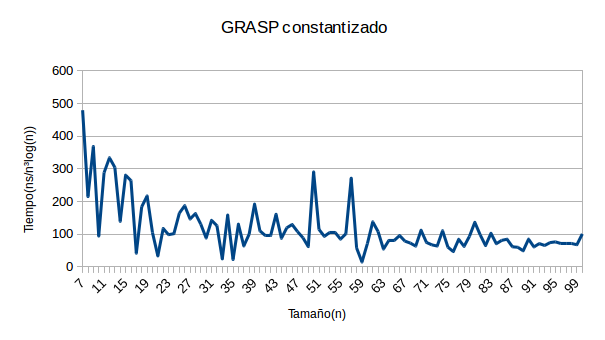
\includegraphics[width=1\textwidth]{grasp_constantizado.png}
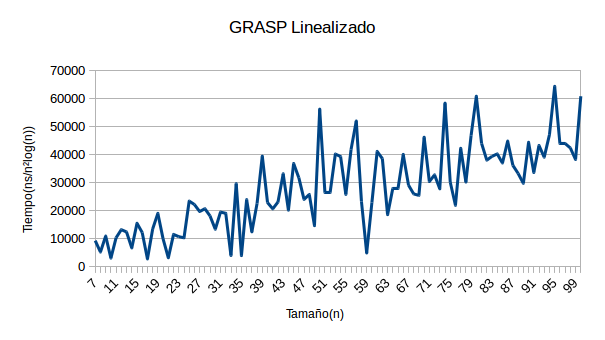
\includegraphics[width=1\textwidth]{grasp_linealizado.png}

Ambos gr�ficos fueron realizados con grafos completos, y por lo tanto $m = \frac{n*(n-1)}{2}$

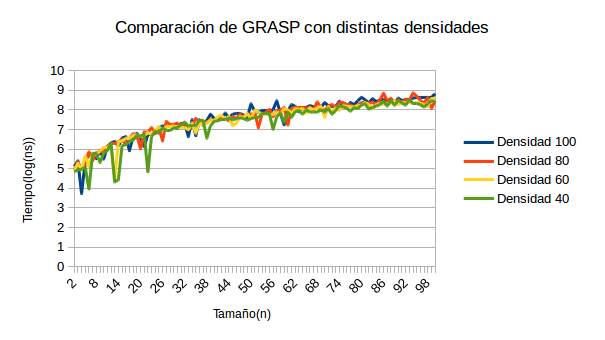
\includegraphics[width=1\textwidth]{densidades_grasp.png}

\subsubsection{Conclusiones}

La experimentaci�n se realiz� con el par�metro $cantIteraciones = 100$, y se dividieron los tiempos de ejecuci�n por la complejidad $O$($cotaIteraciones*(n^3+n*m*(log(n)+log(m))))$).\\

Una observaci�n interesante es que la complejidad de peor caso de nuestro algoritmo es $O$($m*cotaIteraciones*(n^3+n*m*(log(n)+log(m))))$) ya que no es f�cil acotar cuantas veces se correr� el algoritmo de b�squeda
local hasta que no suceda un cambio en $cotaIteraciones$ iteraciones.

Sin embargo en los primeros dos gr�ficos podemos notar que si utilizamos $O$($cotaIteraciones*(n^3+n*m*(log(n)+log(m))))$)
para constantizar y linealizar nos
quedan gr�ficos muy parecidos a los que uno esperar�a si esa fuera su complejidad, por lo que podemos suponer que $O$($cotaIteraciones*(n^3+n*m*(log(n)+log(m))))$) es su complejidad promedio. Tambi�n podr�amos decir
que dadas las mediciones la complejidad del peor caso rara vez se alcanza.\\

En el �ltimo gr�fico, se ve que GRASP corre ligeramente m�s r�pido a menor densidad, aunque la diferencia de tiempo de ejecuci�n entre las distintas densidades es menor que la que uno intuitivamente esperar�a.
Pero tiene sentido al considerar que en el caso promedio el �nico
lugar en el que $m$ aparece en la complejidad del algoritmo es en la b�squeda local, que tiene complejidad $O$($n^3+n*m*log(n)$), dado que $m$ esta acotada por $n^2$ la complejidad se parece mucho independientemente
de el tama�o de la m.

Esto muestra nuevamente que la complejidad de peor caso es una cota muy superior a la complejidad promedio, ya que si la cantidad de ejes afectara tanto a la complejidad deber�a verse reflejada en el ultimo gr�fico.\\

En conclusi�n podr�amos decir que la complejidad verdadera de el algoritmo es mucho mas parecida a $O$($cotaIteraciones*(n^3+n*m*(log(n)+log(m))))$) que a $O$($m*cotaIteraciones*(n^3+n*m*(log(n)+log(m))))$).
\newline

Observaci�n: Para tomar las mediciones, se corre GRASP 20 veces para cada $n$ y se toma el m�nimo de todos esos tiempos, en lugar de hacer un promedio.

\begin{comment}
\newpage
\section{Experimentaci�n General}
\subsection{Generacion de la nueva instancia} 
Para esta parte de la experimentaci�n, creamos nuevas instancias con el generador aleatorio y corrimos la misma instancia con las tres
heur�sticas,
para comparar las soluciones obtenidas y el tiempo de invertido en obtenerlas.

\subsection{Comparaci�n temporal}

A continuaci�n presentamos la comparaci�n temporal entre gr�ficos de distintas densidades. 
L�ase densidad para grafos, como el porcentaje de aristas con respecto al total posible de aristas ($n^2$, con n la cantidad de nodos). 

Respectivamente, los gr�ficos representan las comparaciones para gr�ficos con un 50 $\textperthousand$, 75 $\textperthousand$ y 
100 $\textperthousand$ de aristas. Podemos ver que la relaci�n entre todas se mantiene equivalente.



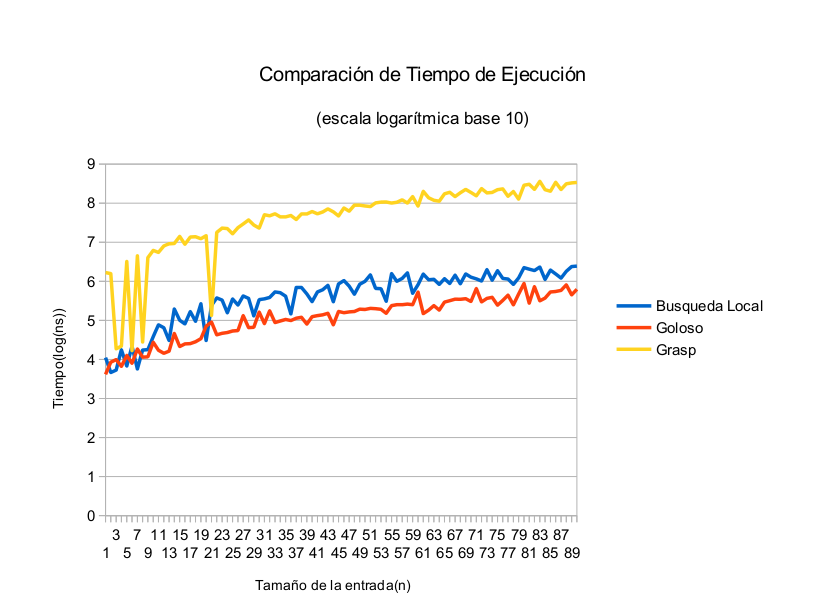
\includegraphics[width=1\textwidth]{heuristicas_grafico_densidad_50.png}

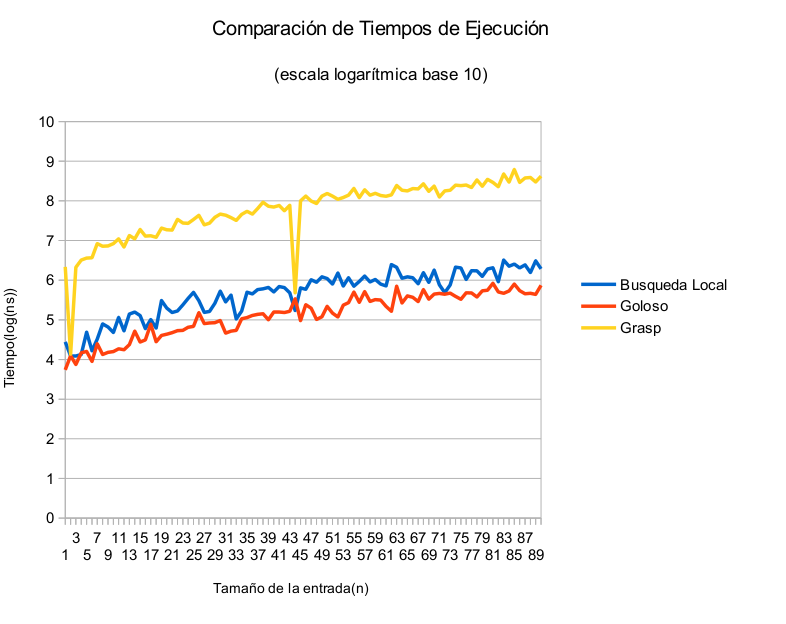
\includegraphics[width=1\textwidth]{heuristicas_grafico_densidad_75.png}

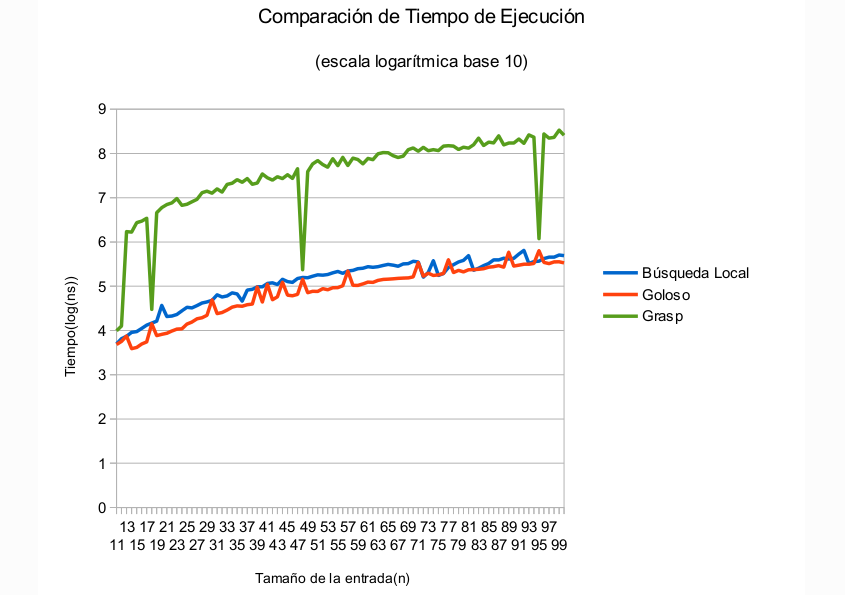
\includegraphics[width=1\textwidth]{heuristicas_grafico_densidad_100.png}



\subsection{Comparaci�n funcional} Comparaci�n entre las respuesta obtenidas.
A continuaci�n presentamos un gr�fico que detalla la diferencia entre los caminos m�nimos obtenidos por cada heur�stica. Como era de 
esperar, la heur�stica Grasp devuelve los caminos de menor peso en la mayor�a de los casos. 

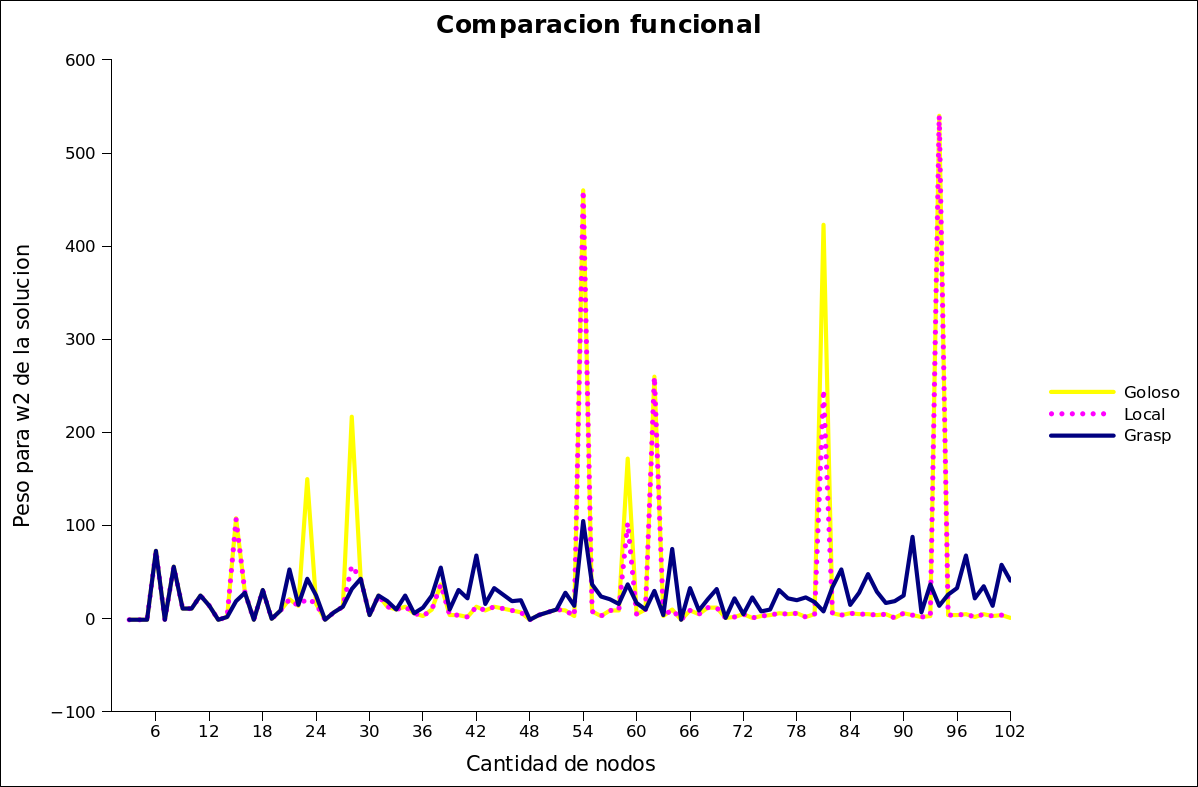
\includegraphics[width=0.8\textwidth]{compFunc}



\subsection{Comparaci�n con la soluci�n �ptima}
A continuaci�n presentamos una tabla que detalla la diferencia entre los caminos m�nimos obtenidos por cada heur�stica comparados con el 
algoritmo exacto. como se puede observar, excepto en las filas con $\sharp$Vertices 9, 13 y 15, las heur�sticas devuelven un resultado 
id�ntico al generado por el algoritmo exacto, esto se debe a que todav�a los grafos son peque�os y es mas probable que las heur�sticas 
encuentren el camino exacto. en las filas con $\sharp$Vertices 9, 13 y 15 es notable la diferencia entre resultados de las heur�sticas, 
dando grasp una soluci�n mucho mejor que las otras dos.
\begin{center}
  \begin{tabular}{| l | c | r | c | r | c | r | c | r | c | r | }
    \hline
	$\sharp$Vertices & $\sharp$Aristas & W2 Exacto & W2 Local & W2 Goloso & W2 Grasp\\ \hline
	1 & 0 & no & no & no & no  \\ \hline
	2 & 1 & 40 & 40 & 40 & 40 \\ \hline
     	3 & 3 & no & no & no & no \\ \hline
	4 & 6 & 25 & 25 & 25 & 25 \\ \hline
	5 & 10 & 54 & 54 & 54 & 54 \\ \hline
	6 & 15 & no & no & no & no \\ \hline
	7 & 21 & 8 & 8 & 8 & 8 \\ \hline
	8 & 28 & no & no & no & no \\ \hline
	9 & 36 & 71 & 238 & 238 & 71 \\ \hline
	10 & 45 & 28 & 28 & 28 & 28 \\ \hline
	11 & 55 & 29 & 29 & 29 & 29 \\ \hline
	12 & 66 & 10 & 10 & 10 & 10 \\ \hline
	13 & 78 & 38 & 111 & 167 & 38 \\ \hline
	14 & 91 & 38 & 38 & 38 & 38 \\ \hline
	15 & 105 & 43 & 107 & 209 & 43 \\ \hline


     \hline
   \end{tabular}
 \end{center}
 


\end{comment}
\end{document}
